\documentclass[]{spie}  %>>> use for US letter paper
%\documentclass[a4paper]{spie}  %>>> use this instead for A4 paper
%\documentclass[nocompress]{spie}  %>>> to avoid compression of citations

\renewcommand{\baselinestretch}{1.0} % Change to 1.65 for double spacing
 
\usepackage{amsmath,amsfonts,amssymb}
\usepackage{graphicx}
\usepackage{algorithm}
\usepackage[noend]{algpseudocode}
\usepackage[colorlinks=true, allcolors=blue]{hyperref}

\title{2D ISAR Modified Orthogonal Matching Pursuit for Doppler-Ambiguous and Off-grid Target Scatterers}

\author[a]{Brandon Boucher}
\author[b]{Mike Davis}
\author[b]{Greg Showman}
\author[b]{Dan Cook}
\author[a]{Justin Romberg}
\affil[a]{Georgia Institute of Technology, 225 North Avenue, Atlanta, US}
\affil[b]{Georgia Tech Research Institute, 250 14th Street, Atlanta, US}

\authorinfo{Further author information: (Send correspondence to Brandon Boucher)\\Brandon Boucher: E-mail: bboucher9@gatech.edu, Telephone: 1 720 443 8892\\  B.B.A.: E-mail: bba@cmp.com, Telephone: +33 (0)1 98 76 54 32}

% Option to view page numbers
\pagestyle{empty} % change to \pagestyle{plain} for page numbers   
\setcounter{page}{301} % Set start page numbering at e.g. 301
 
\begin{document} 
\maketitle

\begin{abstract}
Inverse Synthetic Aperture Radar (ISAR) imaging is advantageous to surveillance and reconnaissance efforts as it enables imaging in any weather, day or night. However, the resolution of the image is dependent on angular diversity and is susceptible to errors from the higher-order motion parameters of a non-cooperative target. For example, if the pulse repetition frequency (PRF) is insufficient to process the incoming Doppler bandwidth of the received echoes, the image can have aliased scatterers. Additionally, target scatterers rarely fit to a defined grid typically used for ISAR imaging, which creates matching basis errors. Though existing methods in literature have demonstrated good reconstruction quality, many have inherent limitations. Learning-based methods require training which can be difficult for ISAR imaging as publicly available real data is scarce. Other methods, like sparse Bayesian learning (SBL) and atomic norm minimization (ANM), are computationally burdensome which can be disadvantageous for imaging platforms with hardware and software limitations or in scenarios where real-time imaging is paramount. Our proposed solution, a modified Orthogonal Matching Pursuit (OMP) algorithm, is able to use the non-uniform motion of the target to aid in disambiguating target scatterers, and our algorithm efficiently finds off-grid target scatterers through Newton’s method. Our algorithm identifies aliased targets in an unambiguous region and determines the originating ambiguity by assessing the correlation of each ambiguous atom with the residual. Our modified OMP processes the latent image in a singular ambiguity as opposed to expanding the sensing matrix to incorporate other ambiguities. This reduces the sensing dictionary dimensionality. From the estimated scattering position, our algorithm then applies Newton’s method in a local neighborhood to refine the off-grid position. Preliminary results demonstrate the algorithm’s effectiveness relative to other modified OMP algorithms, outperforming each in positional accuracy and computational burden.
\end{abstract}

% Include a list of keywords after the abstract 
\keywords{ISAR, doppler ambiguity, non-uniform motion, off-grid}

\section{INTRODUCTION}
\label{sec:intro}  % \label{} allows reference to this section

% motivation and Doppler ambiguity
Inverse synthetic aperture radar (ISAR) imaging enables image creation in all weather systems and is advantageous in many air-to-air and air-to-ground applications. The resolution of an ISAR image is dependent on the bandwidth of the radar in the range direction and the angular diversity of the target in the cross-range direction. Doppler aliasing or Doppler ambiguity arrises when the PRF is less than twice the Doppler frequency of a scatterer. This is a common occurance in applications like space surveillance and imaging of group targets where the far distances necessitates a low PRF or the extension of the target exceeds the Doppler bandwidth <insert references>. The result is ambiguous Doppler frequencies fold into the unambiguous region, where Doppler frequencies originating from ambiguous and unambiguous regions can no longer be differentiated. 

% compressed sensing -> Doppler ambiguity literature review?
Traditionally methods like Time-Frequency analysis and range-Doppler processing are used to address Doppler ambiguities. Another common method is to apply compressed sensing (CS) techniques. CS is a mathematical framework which exploits the sparsity of an image in a sparse domain. CS reduces the dimensionality of the problem from the nullspace of the sensing dictionary to the sparsity. One manifestation of CS are greedy algorithms, in particular OMP, which select atoms from a sensing dictionary with the greatest correlation with the measurement and residual. CS requires the sensing dictionary abides by the Restrictive Isometry Property (RIP) or the coherence requirement <insert citation>. 

The authors of [\citenum{Huang2016}] present a similar methodology to that presented in this paper, applying OMP to form an image by removing the Doppler ambiguity and correcting range cell. Their method leverages the differences in phase progression resulting from range-azimuth coupling and applies OMP to each range cell selecting Fourier-based atoms as a function of Doppler frequency, chirp rate and Doppler ambiguity. Using the selected atoms and subsequently estimated signal parameters, their method removes the Doppler ambiguity and corrects for range cell migration. This method effectively removes Doppler ambiguity; however, their method assumes uniform motion and the scatterers are on-grid. Their method relies on range-azimuth coupling in order disambiguate atoms, which <insert limmitation>. Additionally, because the Doppler ambiguity is included as a dimension in their sensing matrix, the dimensionality and complexity far exceeds our proposed method.


% off-grid
Additionally, ISAR imaging techniques like range-Doppler assume scatterers fall on-grid or at pre-defined range and Doppler combinations. However, real targets do not fall perfectly inline with pre-defined grids, and this descrepancy can cause distortion errors resulting from basis mismatch <insert reference>. The obvious fix is to increase the number of grid points, thereby distributing the energy of the measured reflectivity in a more exact position. This method has drawbacks, and is typically limited by both the additional computation required by increasing the dimensionality of the problem and by the increase in the coherence of atoms if using CS methods.

% Modern off-grid methods
% NOMP, PROMP, SBL, ANM and Learning-based



% doppler ambiguity
% compressed sensing and keystone transform

 

% Doppler ambiguity + off-grid current literature

% Existing modified OMP algorithms

\subsection{Contributions}

The goal of this paper is to leverage non-uniform phase progression to differentiate unambiguous and ambiguous target scatterers. Additionally, our formulation of the problem naturally enables off-grid scatterer compensation where we apply Newton's method to a local neighborhood surrounding a candidate atom. Our key contributions are:

\begin{enumerate}
    \item Our proposed method ModOMP is able to reconstruct ISAR images formed from off-grid scatterers with non-uniform rotation.
    \item We demonstrate the superiority of our method relative to other compressed sensing techniques, and compare reasonably to more computationally burdensome algorithms like SBL and ANM.
    \item We define a performance metric by which we can compare the outputs of ISAR images with strong individual scatterers.
\end{enumerate}

\section{BACKGROUND}

ISAR imaging requires translational motion compensation and rotational motion compensation. Translational motion compensation is typically regarded as trivial and does not add anything outside of undesirable blurring. Assuming the translational motion compensation has been appropriately applied, Figure \ref{fig:geo} depicts the geometry of the target during ISAR imaging where the target is rotating between pulses.

\subsection{Target Geometry}

The crossrange resolution of ISAR images is dictated by the rotation of the target. Assuming translational motion compensation has been applied, this reduces the ISAR model to a tabletop, where the target rotates at a fixed position away from the radar. Additionally, for the purposes of specifically evaluating the effects of non-uniform sampling and slow-time undersampling, the rotation motion parameters are assumed to be known. Figure \ref{fig:geo} depicts the ISAR imaging geometry.

\begin{figure}[h]
  \centering
  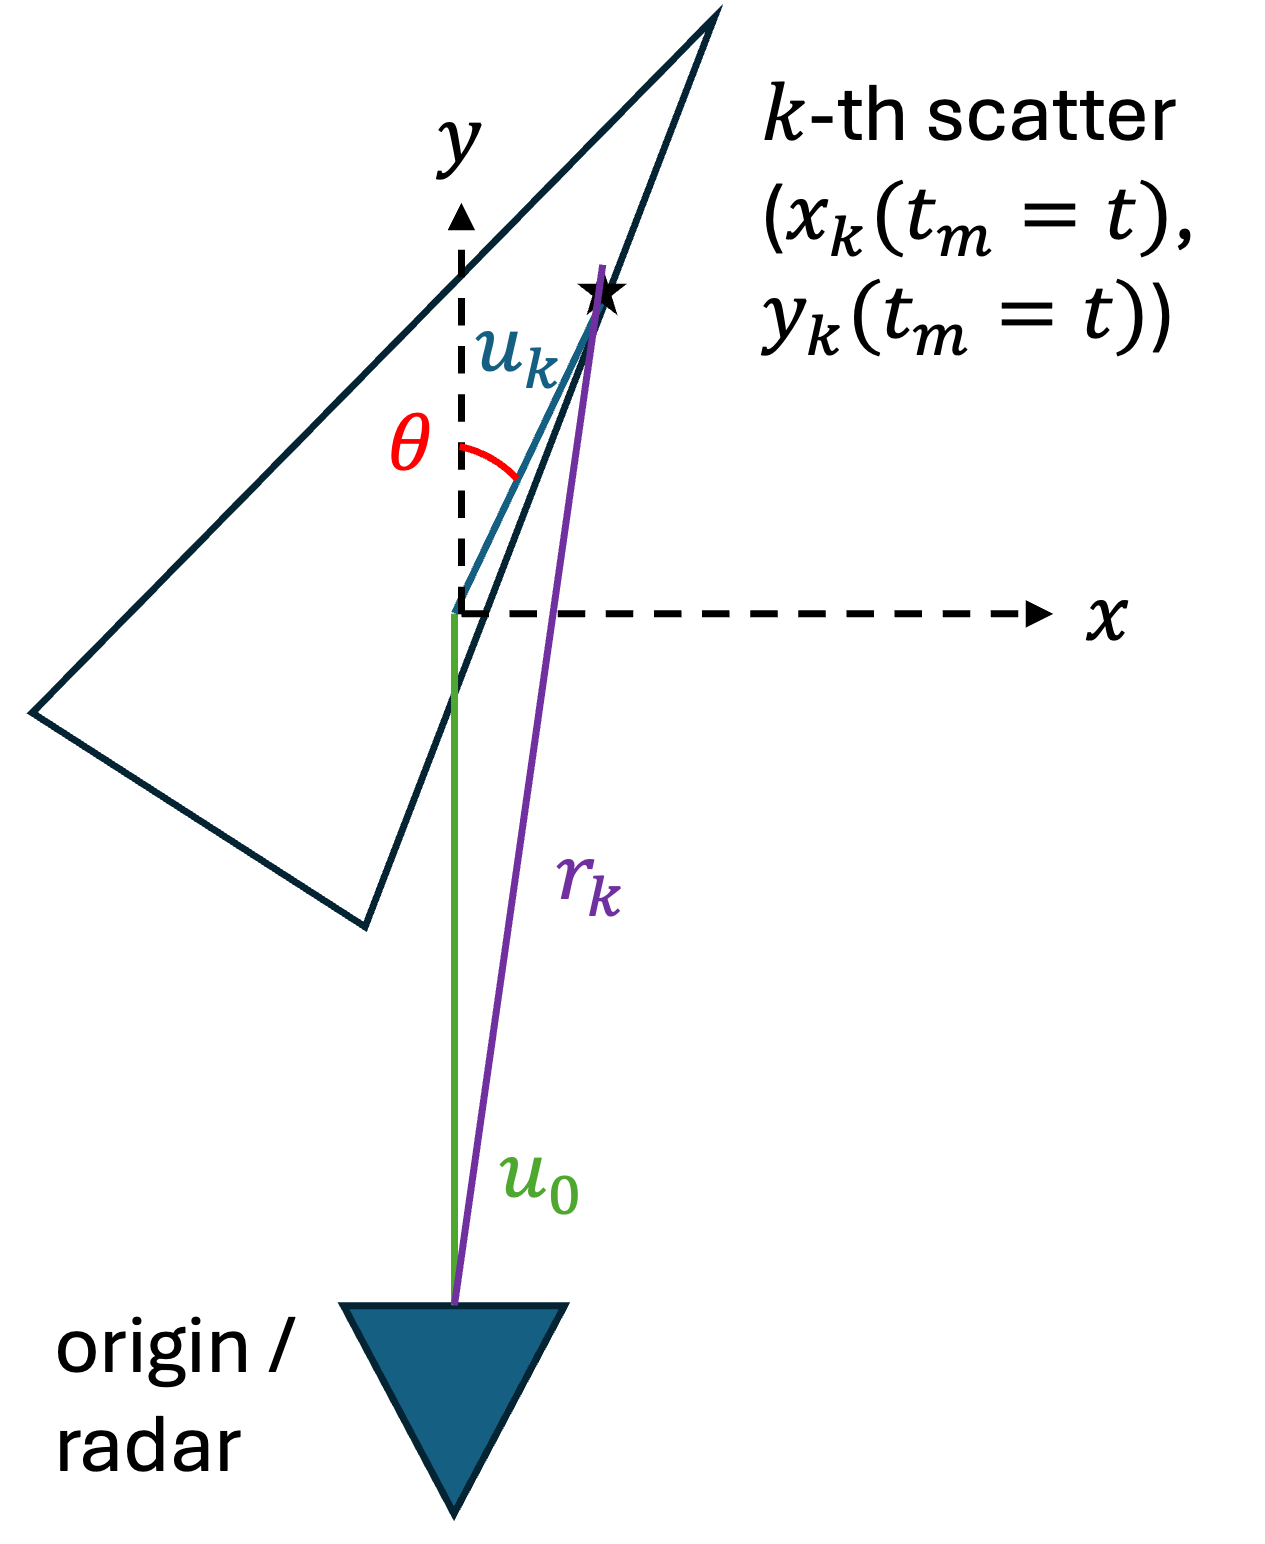
\includegraphics[width=0.3\linewidth]{figures/isar_geo2.png}
  \caption{ISAR target geometry as a function of slow-time}
  \label{fig:geo}
\end{figure}

\noindent The relative position of a scattering point as a function of slow-time ($t_{m}$) can be defined as \cite{Xu2022}:

\begin{equation}
    \begin{bmatrix}
        x_{k}(t_m)\\
        y_k (t_m)
    \end{bmatrix}
    =
    \begin{bmatrix}
        \cos(\theta(t_m)) & -\sin(\theta(t_{m})) \\
        \sin(\theta(t_m)) & \cos(\theta(t_m))
    \end{bmatrix}
    \begin{bmatrix}
        x_{k}\\
        y_k
    \end{bmatrix}
\end{equation}


\noindent where $\theta(t_{m})$ or $\theta_m$ is the angle of the target scatterer relative to the $y$-axis, and $[x_{k}, y_{k}]^{T}$ is the initial position of the $k$-th scatterer relative to the center of the rotation of the target. The range from the origin located at the radar to a scattering point is \cite{Xu2022}:
\begin{equation}
    \begin{aligned}
        r_{k}(t_m) &= \sqrt{x_{k}^2(t_m) + (y_k(t_{m}) + u_{0})^2}\\
        &\approx u_{0} + y_{k}(t_m) \quad \mathrm{as} \quad (y_k(t_{m}) + u_{0})^2 >> x_{k}^2(t_m)\\
        &= u_{0} + x_{k} \sin(\theta(t_{m})) + y_{k}\cos(\theta(t_{m}))\\
        &= u_{0} + u_{k} \\ &\mathrm{where} \quad u_{k} = x_{k} \sin(\theta(t_{m})) + y_{k}\cos(\theta(t_{m}))
    \end{aligned} 
    \label{eq:r}
\end{equation}

\noindent The angle $\theta_m$ can be approximated using a Taylor series:

\begin{equation}
    \begin{aligned}
        \sin(\theta) &= \theta - \frac{\theta^3}{3!} + \frac{\theta^{5}}{5!} + \dots \\
        \cos(\theta) &= 1 - \frac{\theta^2}{2!} + \frac{\theta^{4}}{4!} + \dots
    \end{aligned}
\end{equation}

\noindent For most ISAR applications, the target's rotation is relatively small across the coherent integration time, enabling the usage of the small angle approximation: $\sin(\theta(t_{m})) \approx\theta(t_{m})$ and $\cos(\theta(t_m)) \approx 1$. The range from the radar to a target scatterer can be approximated as:

\begin{equation}
  \begin{aligned}
    r_{k}(t_{m}) &\approx u_{0} + y_{k} + x_{k}\theta_{m} \\ \theta(t_{m}) &= \theta(0) + \omega t_{m} + \frac{\dot{\omega}}{2}t_{m}^{2} + \dots
  \end{aligned}
  \label{eq:r_final}
\end{equation}

\subsection{Signal Model and Sensing Matrix} \label{sec:signal} 

% target geometry
 The signal can be represented as a range-compressed echo:

\begin{equation}
    s(\hat{t},t_{m}) = C \cdot \text{sinc}(B(\hat{t} - \tau(t_{m})))\cdot \exp(-j2 \pi f_{c} \tau(t_{m}))
\end{equation}

\noindent where $C$ is the amplitude, $B$ is the bandwidth, $\hat{t}$ is the fast-time, $t_{m}$ is the slow-time, $\tau$ is the propagation delay and $f_{c}$ is the center frequency. The propagation delay for a monostatic radar configuration is the amount of time required to propagate to the target and return:

\begin{equation}
    \tau_{m} = \frac{2r(t_{m})}{c}
\end{equation}

\noindent where $r(t_{m})$ is the range or distance from the radar to a target scattering point as defined by equation \ref{eq:r}. The return echo can be represented as a summation of the returns from each scatterer:

\begin{equation}
    s(\hat{t},t_{m}) = C \sum_{k} \sigma_{k} \cdot \delta(\hat{t} - \tau_{k}(t_{m})) \cdot \exp(-j2 \pi f_{c} \tau_{k}(t_{m}))
\end{equation}

\noindent where $k$ is the index of each scatterer located at $\delta(\hat{t} - \tau_{k}(t_{m}))$, $K$ is the total number of scatterers or sparsity, and $\sigma_{k}$ is the complex reflectivity of the $k$-th scatterer. Typical formulations will assume separability in the range and crossrange to simplify the sensing matrix's formulation; however, this approach neglects the cross-terms inherent to range-cell migration. To preserve this effect while still defining a linear system suitable for reconstruction using compressed sensing, apply the Fourier transform in the fast-time:

\begin{equation}
    S(\hat{f},t_{m}) = C \sum_{k} \sigma_{k} \cdot \exp(-j2 \pi (f_{c} + \hat{f}) \tau_{k}(t_{m}))
    \label{eq:S}
\end{equation}

\noindent where $\hat{f}$ is the temporal-frequency or the range-frequency. Equation \ref{eq:S} enables a formulation of a sensing matrix where each entry can be defined as:

\begin{equation}
    A[{m + \ell M}, k] = C \sigma_{k} \cdot \exp(-j2 \pi (f_{c} + \hat{f}_{\ell}) \tau_{k}(t_{m}))
\end{equation}

\noindent The resulting linear system is defined as: $y = Ax + n$, where $y \in \mathbb{C}^{ML}$ is the measurement, $A \in \mathbb{C}^{ML \times K}$ is the sensing matrix, and $x \in \mathbb{C}^{K}$ is the vectorized latent image. The dimensionality of the system is determined by the number of range-frequency samples $L$, the number of scatterers $K$ and the number of received pulses $M$ which is less than the number of total pulses $N$ such that $M << N$. Figure \ref{fig:sensing_matrix} depicts the dimensionality of the proposed sensing matrix. 

\begin{figure}[h]
  \centering
  
\includegraphics[width=0.4\linewidth]{figures/linear_sys1.png}
  \caption{Linear system formulation and dimensionality}
  \label{fig:sensing_matrix}
\end{figure}

This system is underdetermined and has infinitely many solutions, each existing in the ($N-M$)-dimensional null space of the sensing matrix. However, to treat this as a compressed sensing problem, if the latent image can be assumed $K$-sparse or containing $K$ non-zero values, the problem becomes $K$-dimensional where $M \geq K$. Additionally, if the sensing matrix is roughly orthogonal and incoherent, associated with the Restricted Isometric Property (RIP), the solution can be unique \cite{Majumdar_2018}. The compressed sensing problem can then be formulated as:

\begin{equation}
    \min_{x} ||x||_{0} \quad \text{subject to} \quad y = Ax
    \label{eq:l0}
\end{equation}

There are many different compressed sensing techniques, and Greedy algorithms like Orthogonal Matching Pursuit (OMP) are effective for non-linear recovery \cite{Bostock_2017}. For a Hermitian sensing matrix ($A$) where $A^{-1} = A^{H}$, OMP iterates through a defined sparsity ($K$) and finds the indices ($\Lambda$) that maximize the projection of the residual, initialized as the measurement, onto the basis vectors formed by $A$. The maximization of the residual selects the coefficients projected on the basis vectors formed by $A$, and the step $r = y - A \hat{X}$ prevents the re-selection of the same indices. The latent image estimation $\hat{X}$ is the least-squares approximation formed from the selected basis vectors of $A$. Algorithm \ref{algo:OMP} formally describes the OMP algorithm \cite{Majumdar_2018}.

\begin{algorithm}[H]
\caption{Orthogonal Matching Pursuit}\label{algo:OMP}
\begin{algorithmic}[1]
\Procedure{OMP}{$H,N$}
\State $\Lambda\gets []$
\State $r \gets y$
\State $\hat{X} \gets 0$
\For{$i \leq K$}
\State $c\gets A^{H}r$
\State $\Lambda = \arg\max_{i} \big| c_i \big|$
\State $\Lambda \gets \begin{bmatrix} \Lambda \\ l \end{bmatrix}$
\State $\hat{X} \gets (A(\Lambda)^{H}A(\Lambda))^{-1}A(\Lambda)^{H}y$
\State $r \gets y - A\hat{X}$
\State $i \gets i + 1$
\EndFor
\State \textbf{return} $\hat{X}$
\EndProcedure
\end{algorithmic}
\end{algorithm}

\section{Modified OMP}

% non-uniform phase progression -> atom differentiation
The resolution of an ISAR image is dependent on the bandwidth of the radar and the rotation of the target. As the target rotates and the integration angle increases, the cross range resolution of the target improves. However, in applications like air-to-air detection, classification and tracking, the target's motion is typically complex and has high-order motion parameters, rotational acceleration, jerk, etc \cite{Liu_2012}. Traditionally these higher-order motion parameters are seen as a nuisance as they can corrupt and contaminate the image formation process with unwanted phase errors. However, higher-order motion parameters also introduce non-uniform phase progression or non-uniform sampling, which can be advantageous in differentiating otherwise highly correlated scatterers.

\subsection{Complexity}

\section{Results}



\section{Discussion}

\section{Conclusion}

% References
\bibliography{bib} % bibliography data in report.bib
\bibliographystyle{spiebib} % makes bibtex use spiebib.bst

\end{document} 
